\chapter{Implementazione}
Una volta definita la vista generale del progetto possiamo passare alla fase implementativa. Si è deciso di utilizzare Java per la soluzione in maniera tale da mantenere una certa continuità con Tint e con SimpleNLG.\\
\section{Costruzione struttura dati sintattica}
Per costruire l'albero si sono utilizzate le informazioni provenienti dal JSON prodotto da Tint. Infatti, ogni nodo dell'albero presenta queste informazioni; tale scelta è dovuta anche al fatto che, in caso ci siano due occorrenze della stessa parola nella frase, si presenta la possibilità per il sistema di effettuare una discriminazione tra le occorrenze stesse. La struttura è la seguente.\\
\begin{figure}[h!]
	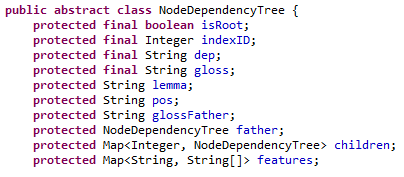
\includegraphics[scale=0.55]{StrutturaDati.PNG}
	\centering
	\caption{Struttura dati utilizzata}
	\label{fig:PM}
\end{figure}
\clearpage
Per prima cosa occorre definire i controlli implementati in base alle dipendenze trovate dopo la fase di parsing delle 3 frasi. Le dipendenze sono:
\begin{itemize}
	\item \textbf{aux}: indica la presenza di un verbo ausiliare, modifica le informazioni relative ad un predicato verbale come il tempo/modo;
	\item \textbf{auxpass}: indica la presenza di un verbo di forma passiva, permettendoci di capire se
	rendere True o False la ‘Feature.PASSIVE’ del verbo;
	\item \textbf{cop}: indica la presenza di un verbo copulativo. Il nodo figlio, a differenza del caso
	‘aux’ è il verbo da settare, ma come in ‘aux’, useremo i dati morfologici legati al
	suddetto nodo per il tempo e la persona.
	\item \textbf{advmod}: indica la presenza di un avverbio, dunque viene modificata la VP, concatenando l’avverbio al verbo mediante il metodo addModifier("avverbio"). In questo modo riusciamo ad ottenere una traduzione più fedele;
	\item \textbf{det/det-poss}: indica un determiner. Se esiste una NP(nounPhrase) viene passato come parametro alla funzione che crea NP. Ad esempio, nlgFactory.createNounPhrase("determiner", "parola");
	\item \textbf{compound}: indica la presenza di un sostantivo composto (spada laser). Anche in questo caso utilizzeremo la funzione addModifier();
	\item \textbf{case}: indica il collegamento con una prepositional phrase;
	\item \textbf{amod}: indica la presenza di un aggettivo modificatore. Si aggiunge come pre modifier “addPreModifier()”;
	\item \textbf{nsubjpass}: indica la presenza di soggetto in una frase passiva, quindi viene gestito come fosse l’oggetto della frase.
\end{itemize}
Inoltre, occorre effettuare anche dei controlli sul nodo attuale:
\begin{itemize}
	\item \textbf{nmod}: indica l’inizio di una NounPhrase. Indica la presenza del complemento di specificazione del complemento oggetto della frase. Nmod, non è quindi da specificare come un post modifier della clausola, ma come un post modifier della NP di cui è figlio nella dipendenza;
	\item \textbf{dobj}: indica l’oggetto di una VP(verb phrase), viene istanziato come una NP.
\end{itemize}
Successivamente si è passati alla fase di traduzione. Una volta definite le dipendenze incontrate è stato possibile "posizionare" le componenti della frase al proprio posto. Come possiamo vedere dall'immagine che segue, di fondamentale importanza è la classe \textbf{TransferTranslationItENG} in quanto al suo interno sono stati implementati i controlli sulle dipendenze e le funzioni di traduzione. Da quella poi viene richiamato il \textbf{Realiser} di SimpleNLG per andare a costruire la frase in inglese.  
\begin{figure}[h!]
	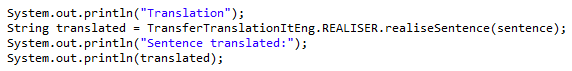
\includegraphics[scale=0.75]{Realiser.PNG}
	\centering
	\caption{Creazione frase tradotta.}
	\label{fig:PM}
\end{figure}
\\
Le traduzioni finali sono state:
\begin{itemize}
	\item è la spada laser di tuo padre - is your father lightsaber;
	\item ha fatto una mossa leale - made a fair move;
	\item Gli avanzi della vecchia Repubblica sono stati spazzati via - The last leftover of the old repubblica have been wiped out.
\end{itemize}
In quest'altra immagine invece viene esplicitato il controllo attraverso cui si va ad aggiungere un aggettivo attraverso il metodo addPreModifier("aggettivo"). Viene presa la parola relativa a quella dipendenza, viene tradotta e poi passata al metodo stesso.
\begin{figure}[h!]
	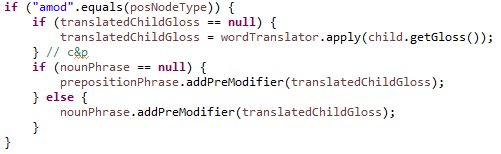
\includegraphics[scale=0.75]{AdjModifier.PNG}
	\centering
	\caption{Controllo sulla dipendenza Amod}
	\label{fig:PM}
\end{figure}
\clearpage
